  \documentclass{article}

\input{"MathTopMatter.tex"}

\usepackage[framed,numbered,autolinebreaks,useliterate]{mcode}

\usepackage{fullpage}

\title{Seperation of Video in Foreground/Background using DMD (AMATH 582 Homework 4)}
\author{Ronan Keane}
\date{4182 W Stephen's Way NE, Room 103, ~Seattle, WA 98105 \\ ~ronank@uw.edu~}

\makeatletter
\newcommand{\rmnum}[1]{\romannumeral #1}
\newcommand{\Rmnum}[1]{\expandafter\@slowromancap\romannumeral #1@}
\makeatother
%\renewcommand{\thesection}{Problem \arabic{section}.}
%\renewcommand{\thesubsection}{\arabic{section} (\alph{subsection})}
%\renewcommand{\thesubsubsection}{\arabic{section} (\alph{subsection}) (\roman{subsubsection})}

%\def\A{
%\begin{bmatrix}
%    x_1 & x_2 & \cdots & x_N
%\end{bmatrix}}

\begin{document}
\maketitle
%figures

\begin{figure}
	\centering
	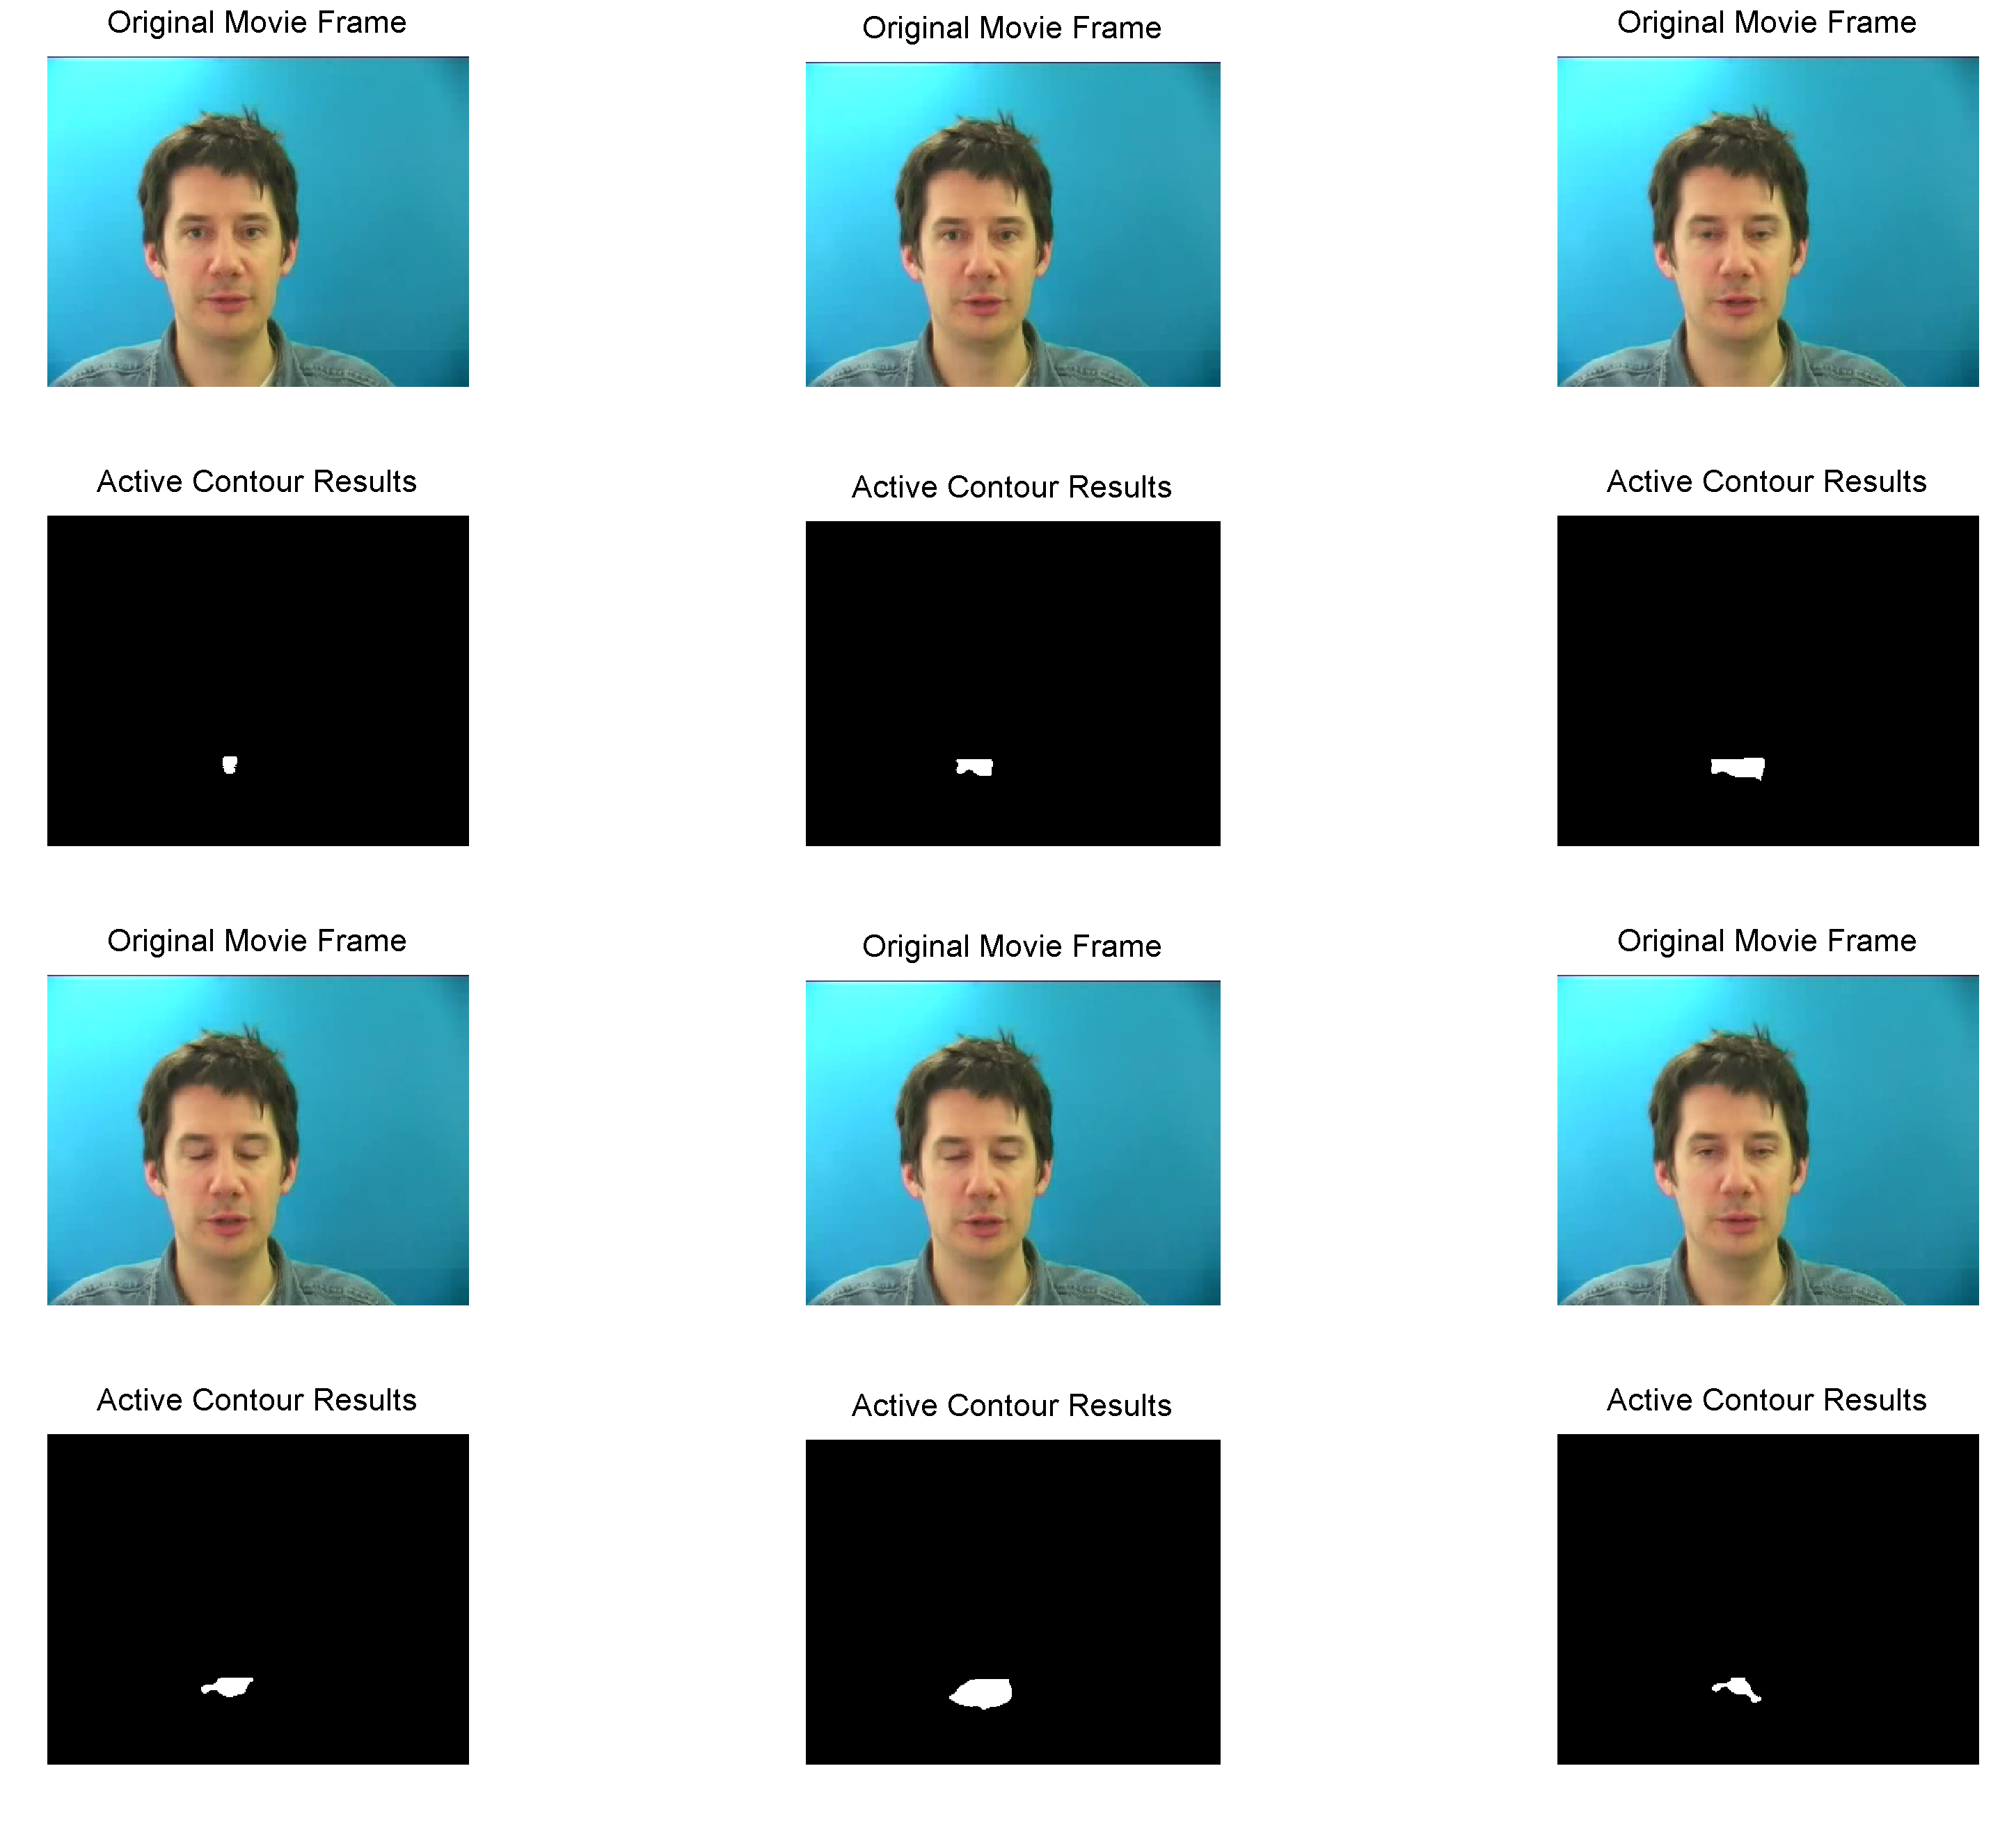
\includegraphics[width=1\textwidth]{AC1.png}
	\caption{Active Contour Results for selected frames. Active contour provides an inconsistent lip profile because it never properly converges.}
\end{figure}

\begin{figure}
	\centering
	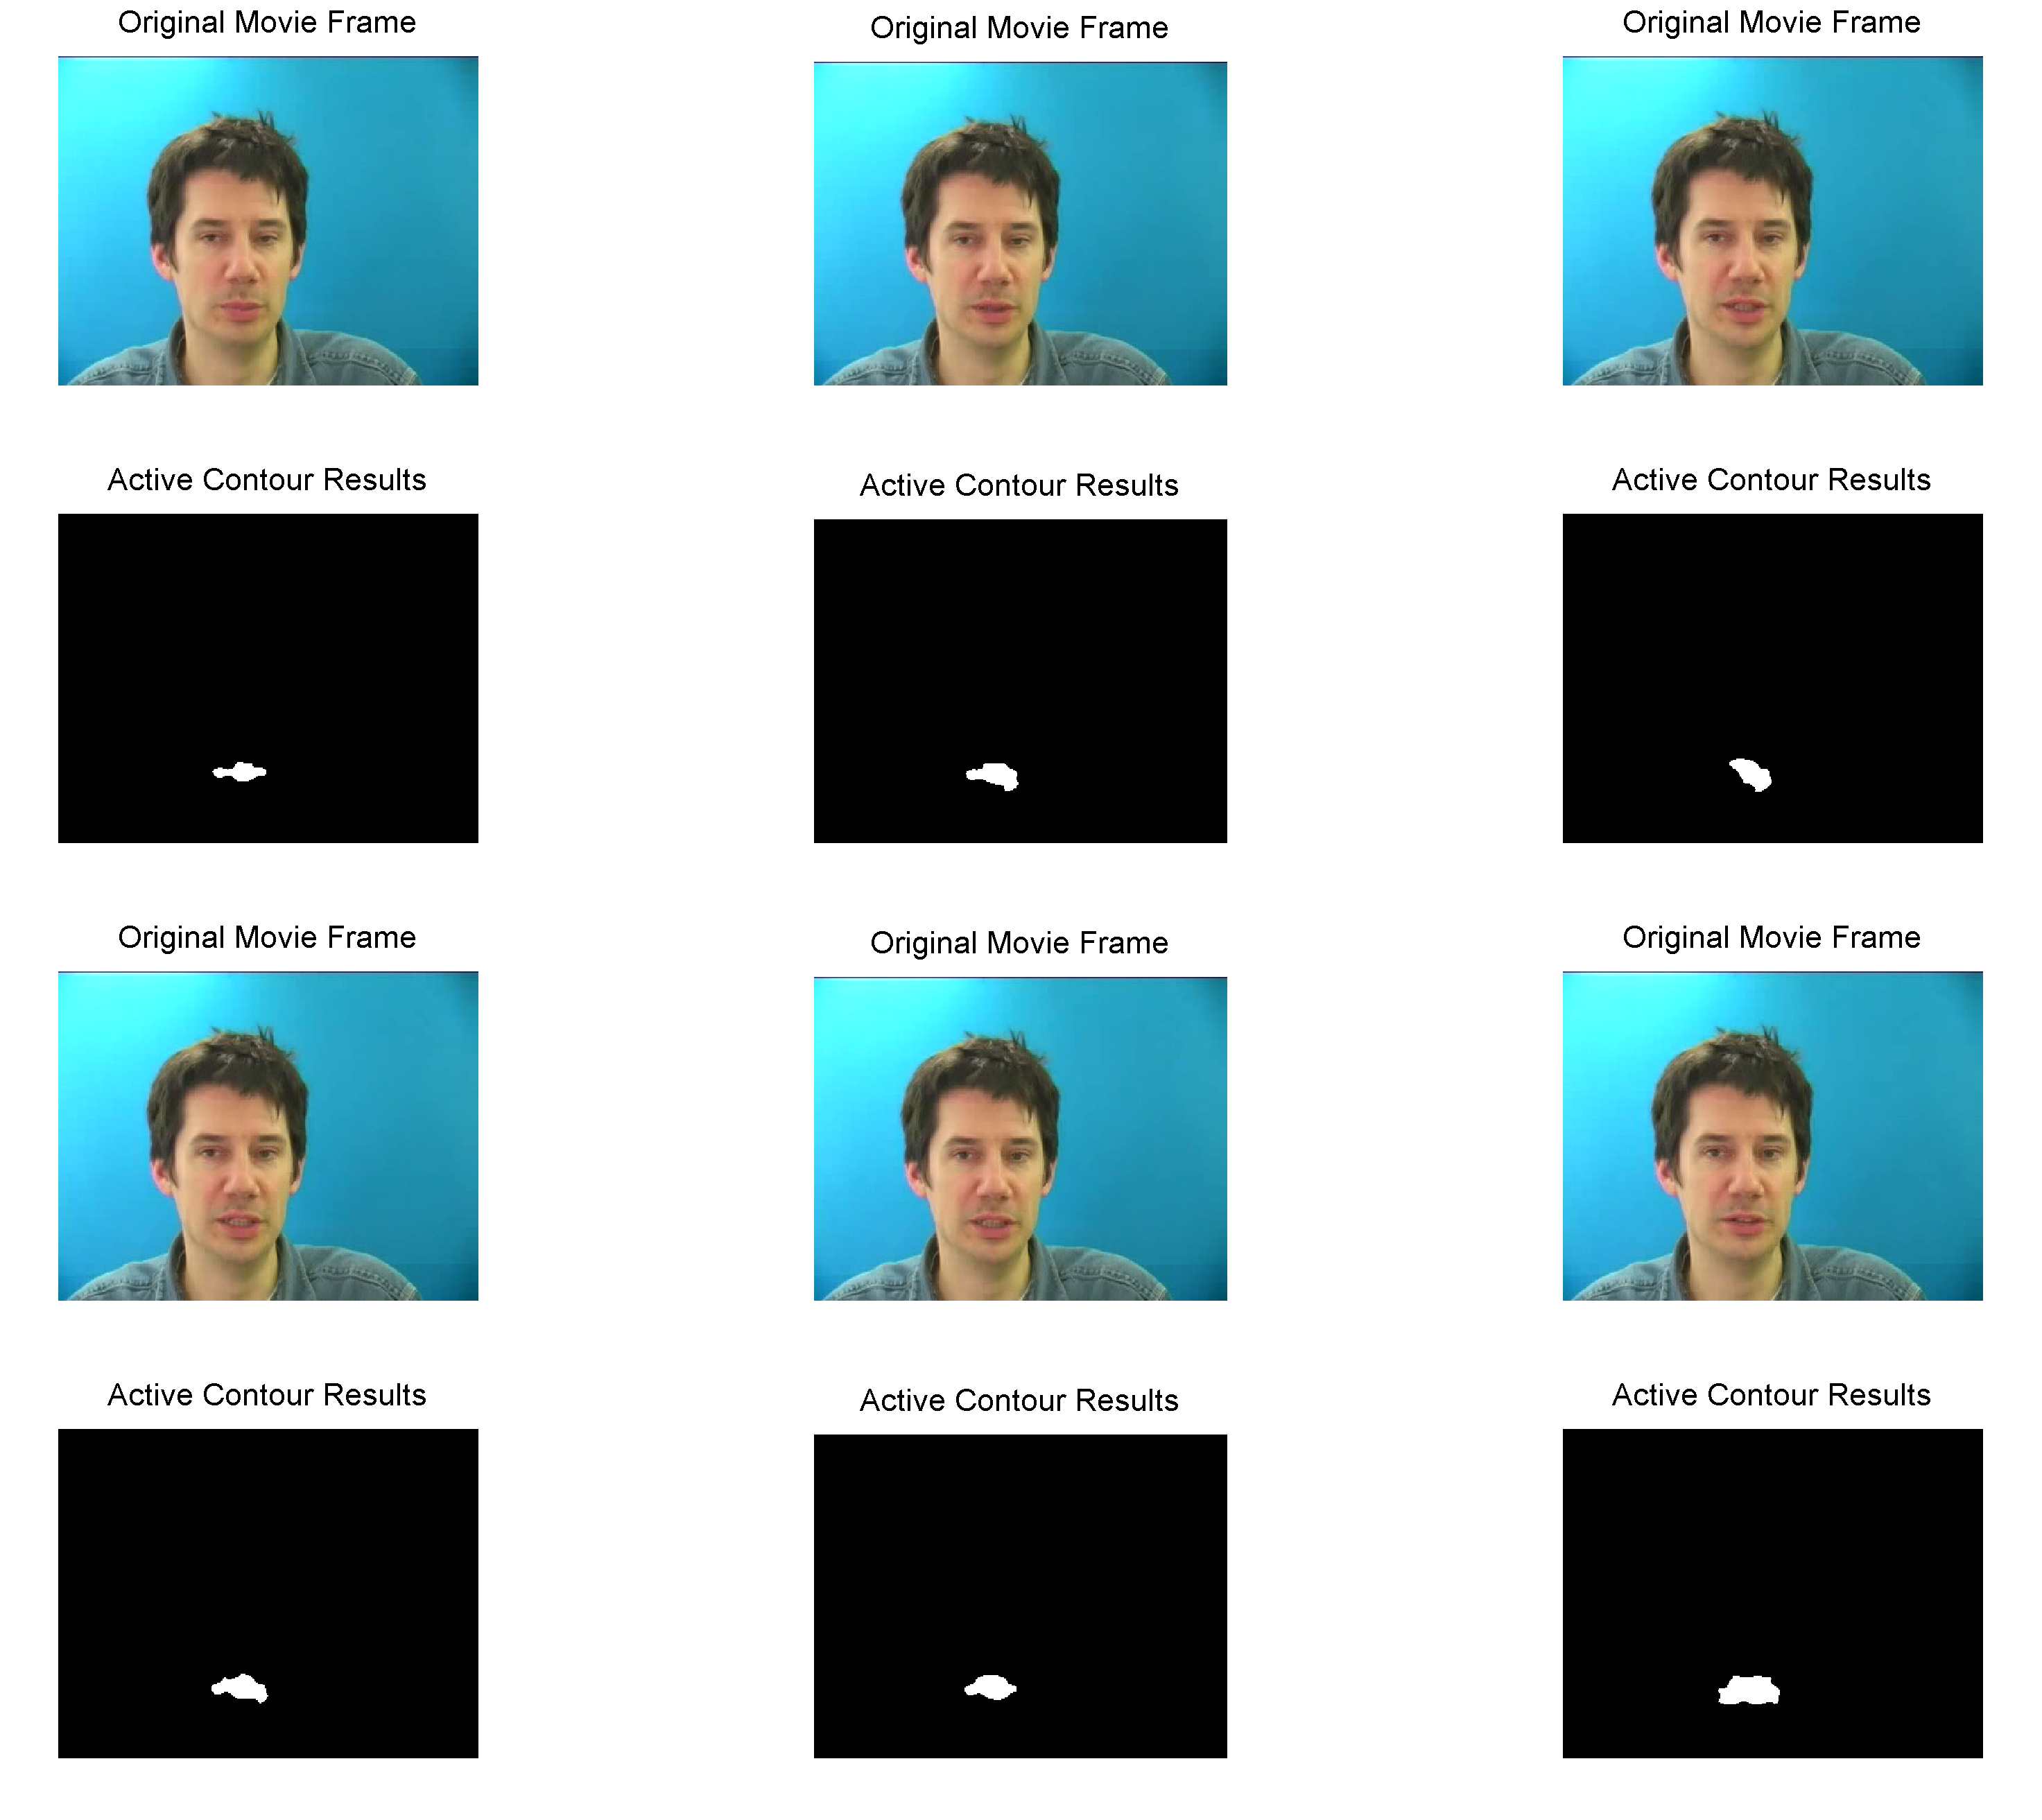
\includegraphics[width=1\textwidth]{AC2.png}
	\caption{Active Contour Results for selected frames. Active contour provides an inconsistent lip profile because it never properly converges.}
\end{figure}

\begin{figure}
	\centering
	\includegraphics[width=1\textwidth]{DMD1.png}
	\caption{DMD results for selected frames. DMD is not ideal in this situation because the background (the man's face) is not completely stationary.}
\end{figure}

\begin{figure}
	\centering
	\includegraphics[width=1\textwidth]{DMD2.png}
	\caption{DMD results for selected frames. DMD is not ideal in this situation because the background (the man's face) is not completely stationary.}
\end{figure}

\begin{figure}
	\centering
	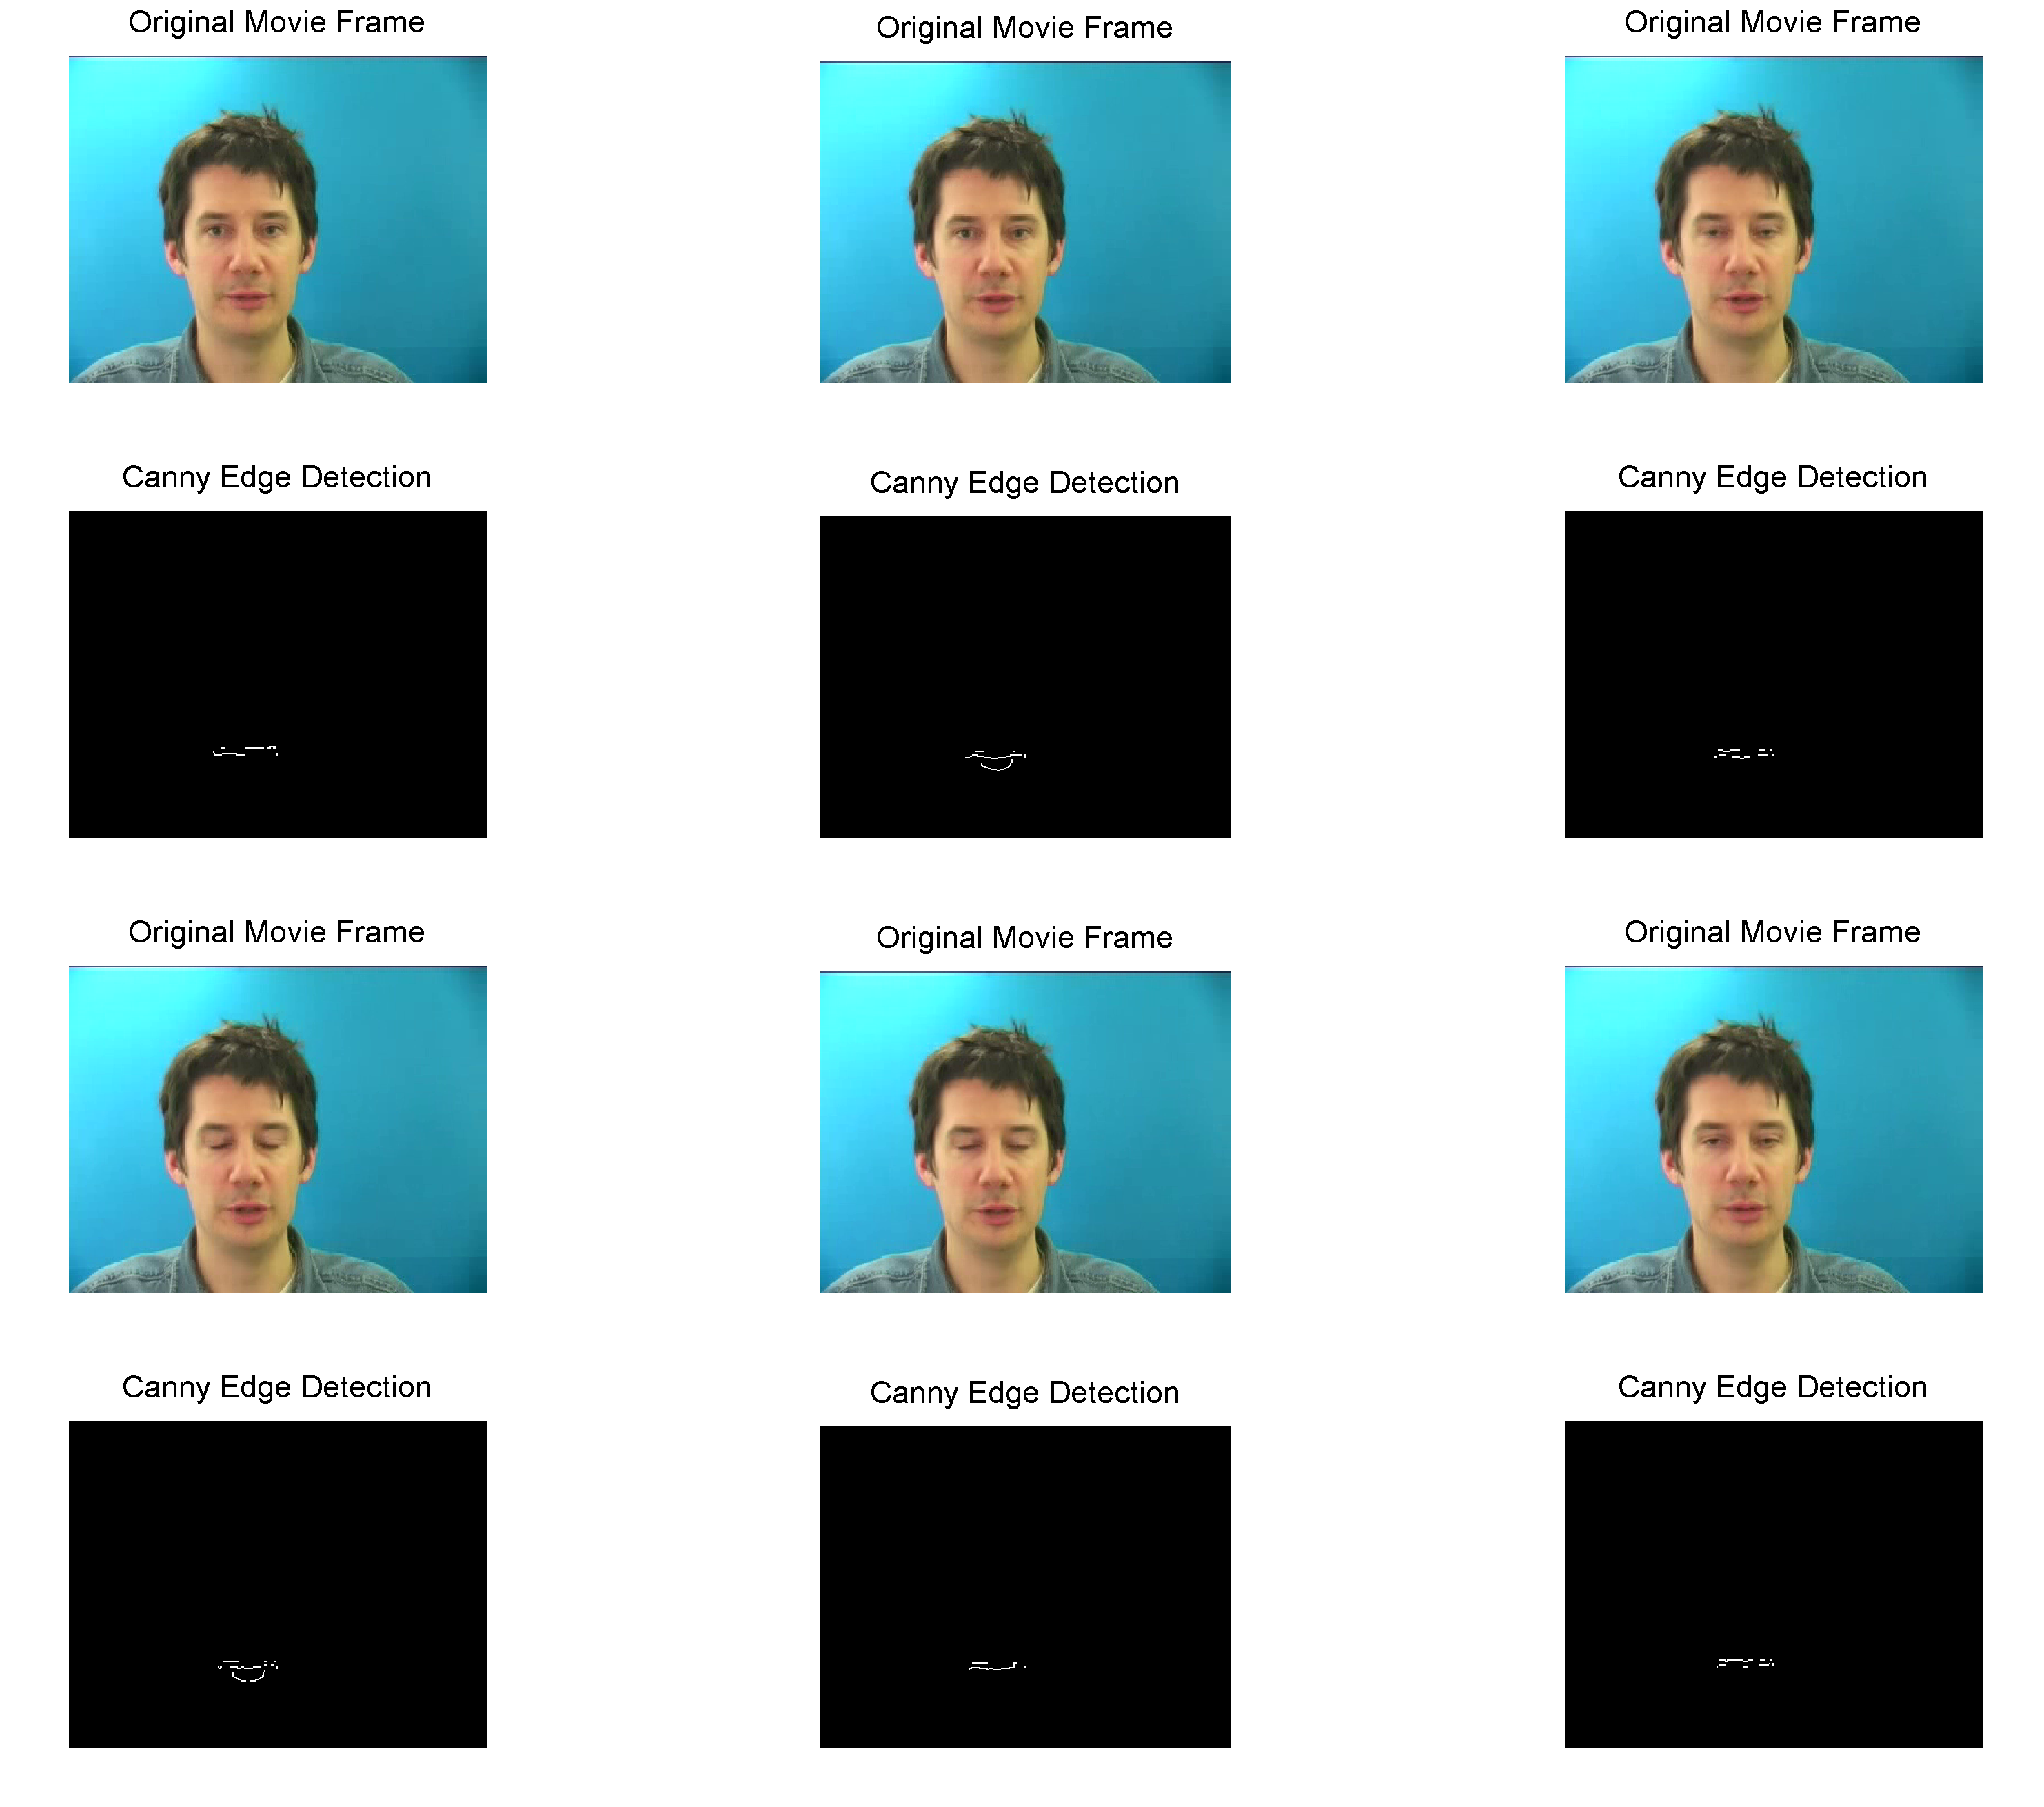
\includegraphics[width=1\textwidth]{canny1.png}
	\caption{Canny Edge Detection results for selected frames. Although it captures the profile of the lips, it does not always capture the entire contour.It also does not show the inside of the lips.}
\end{figure}

\begin{figure}
	\centering
	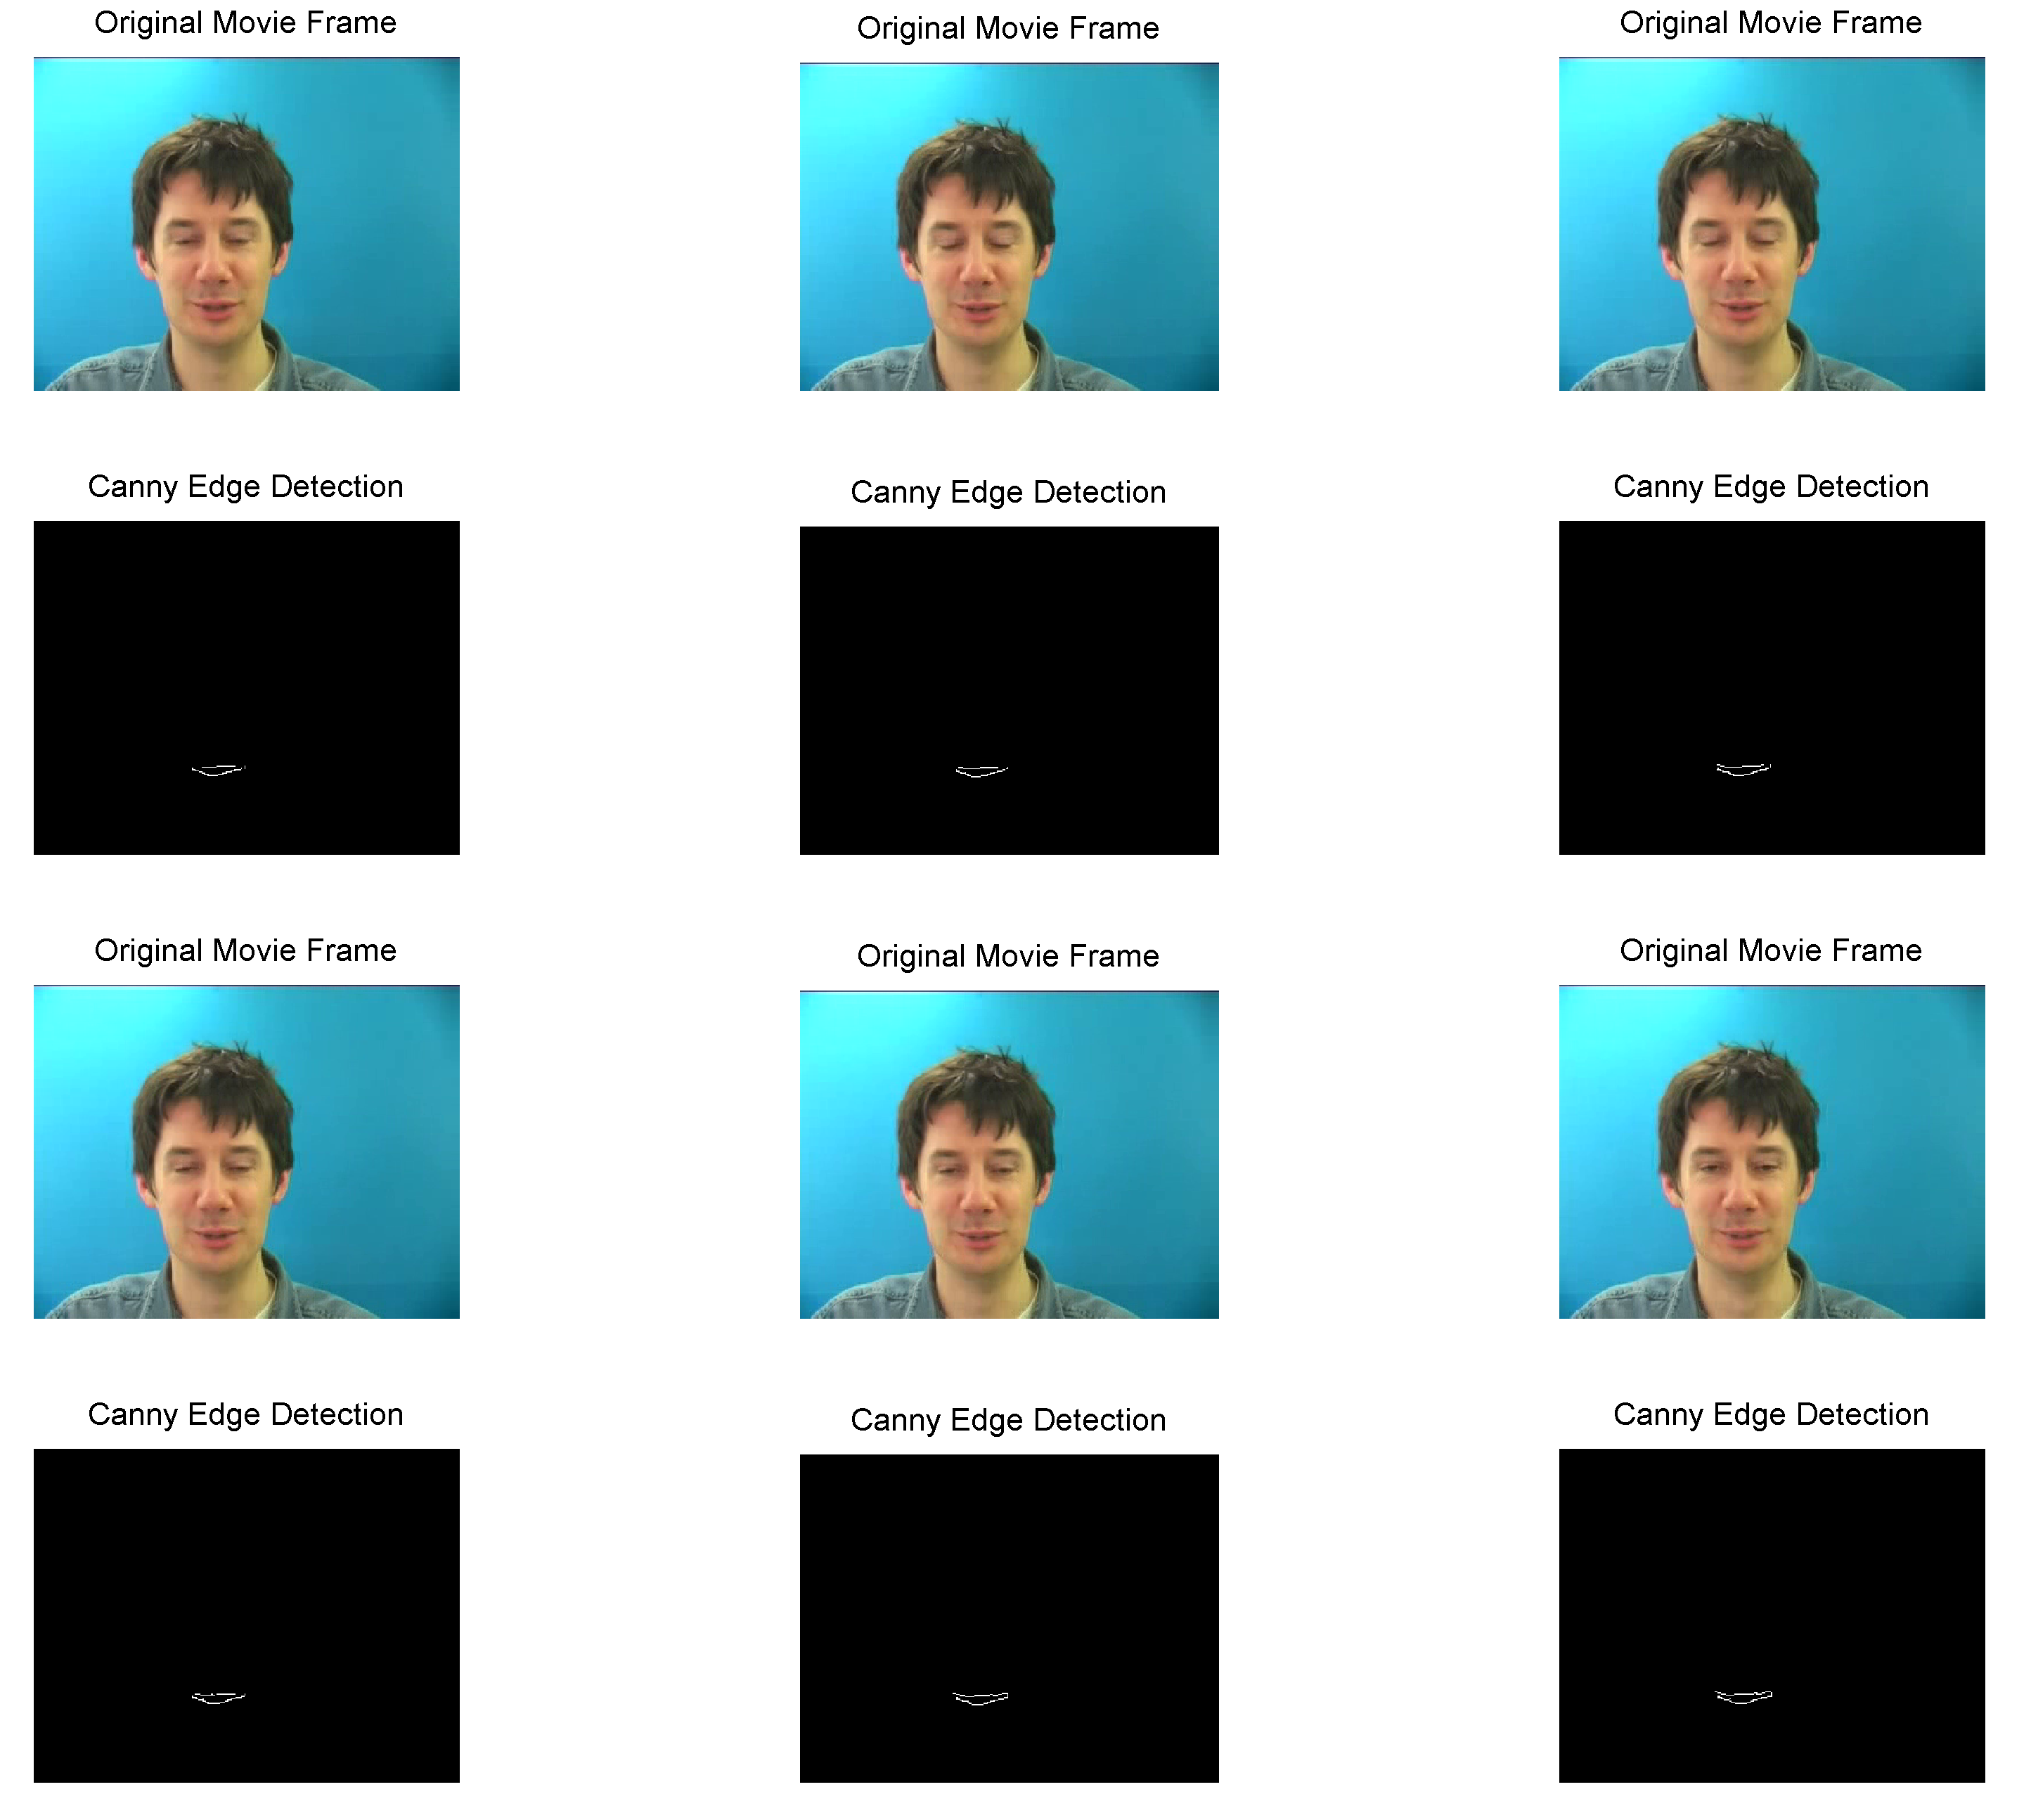
\includegraphics[width=1\textwidth]{canny2.png}
	\caption{Canny Edge Detection results for selected frames. Although it captures the profile of the lips, it does not always capture the entire contour. It also does not show the inside of the lips.}
\end{figure}

\begin{figure}
	\centering
	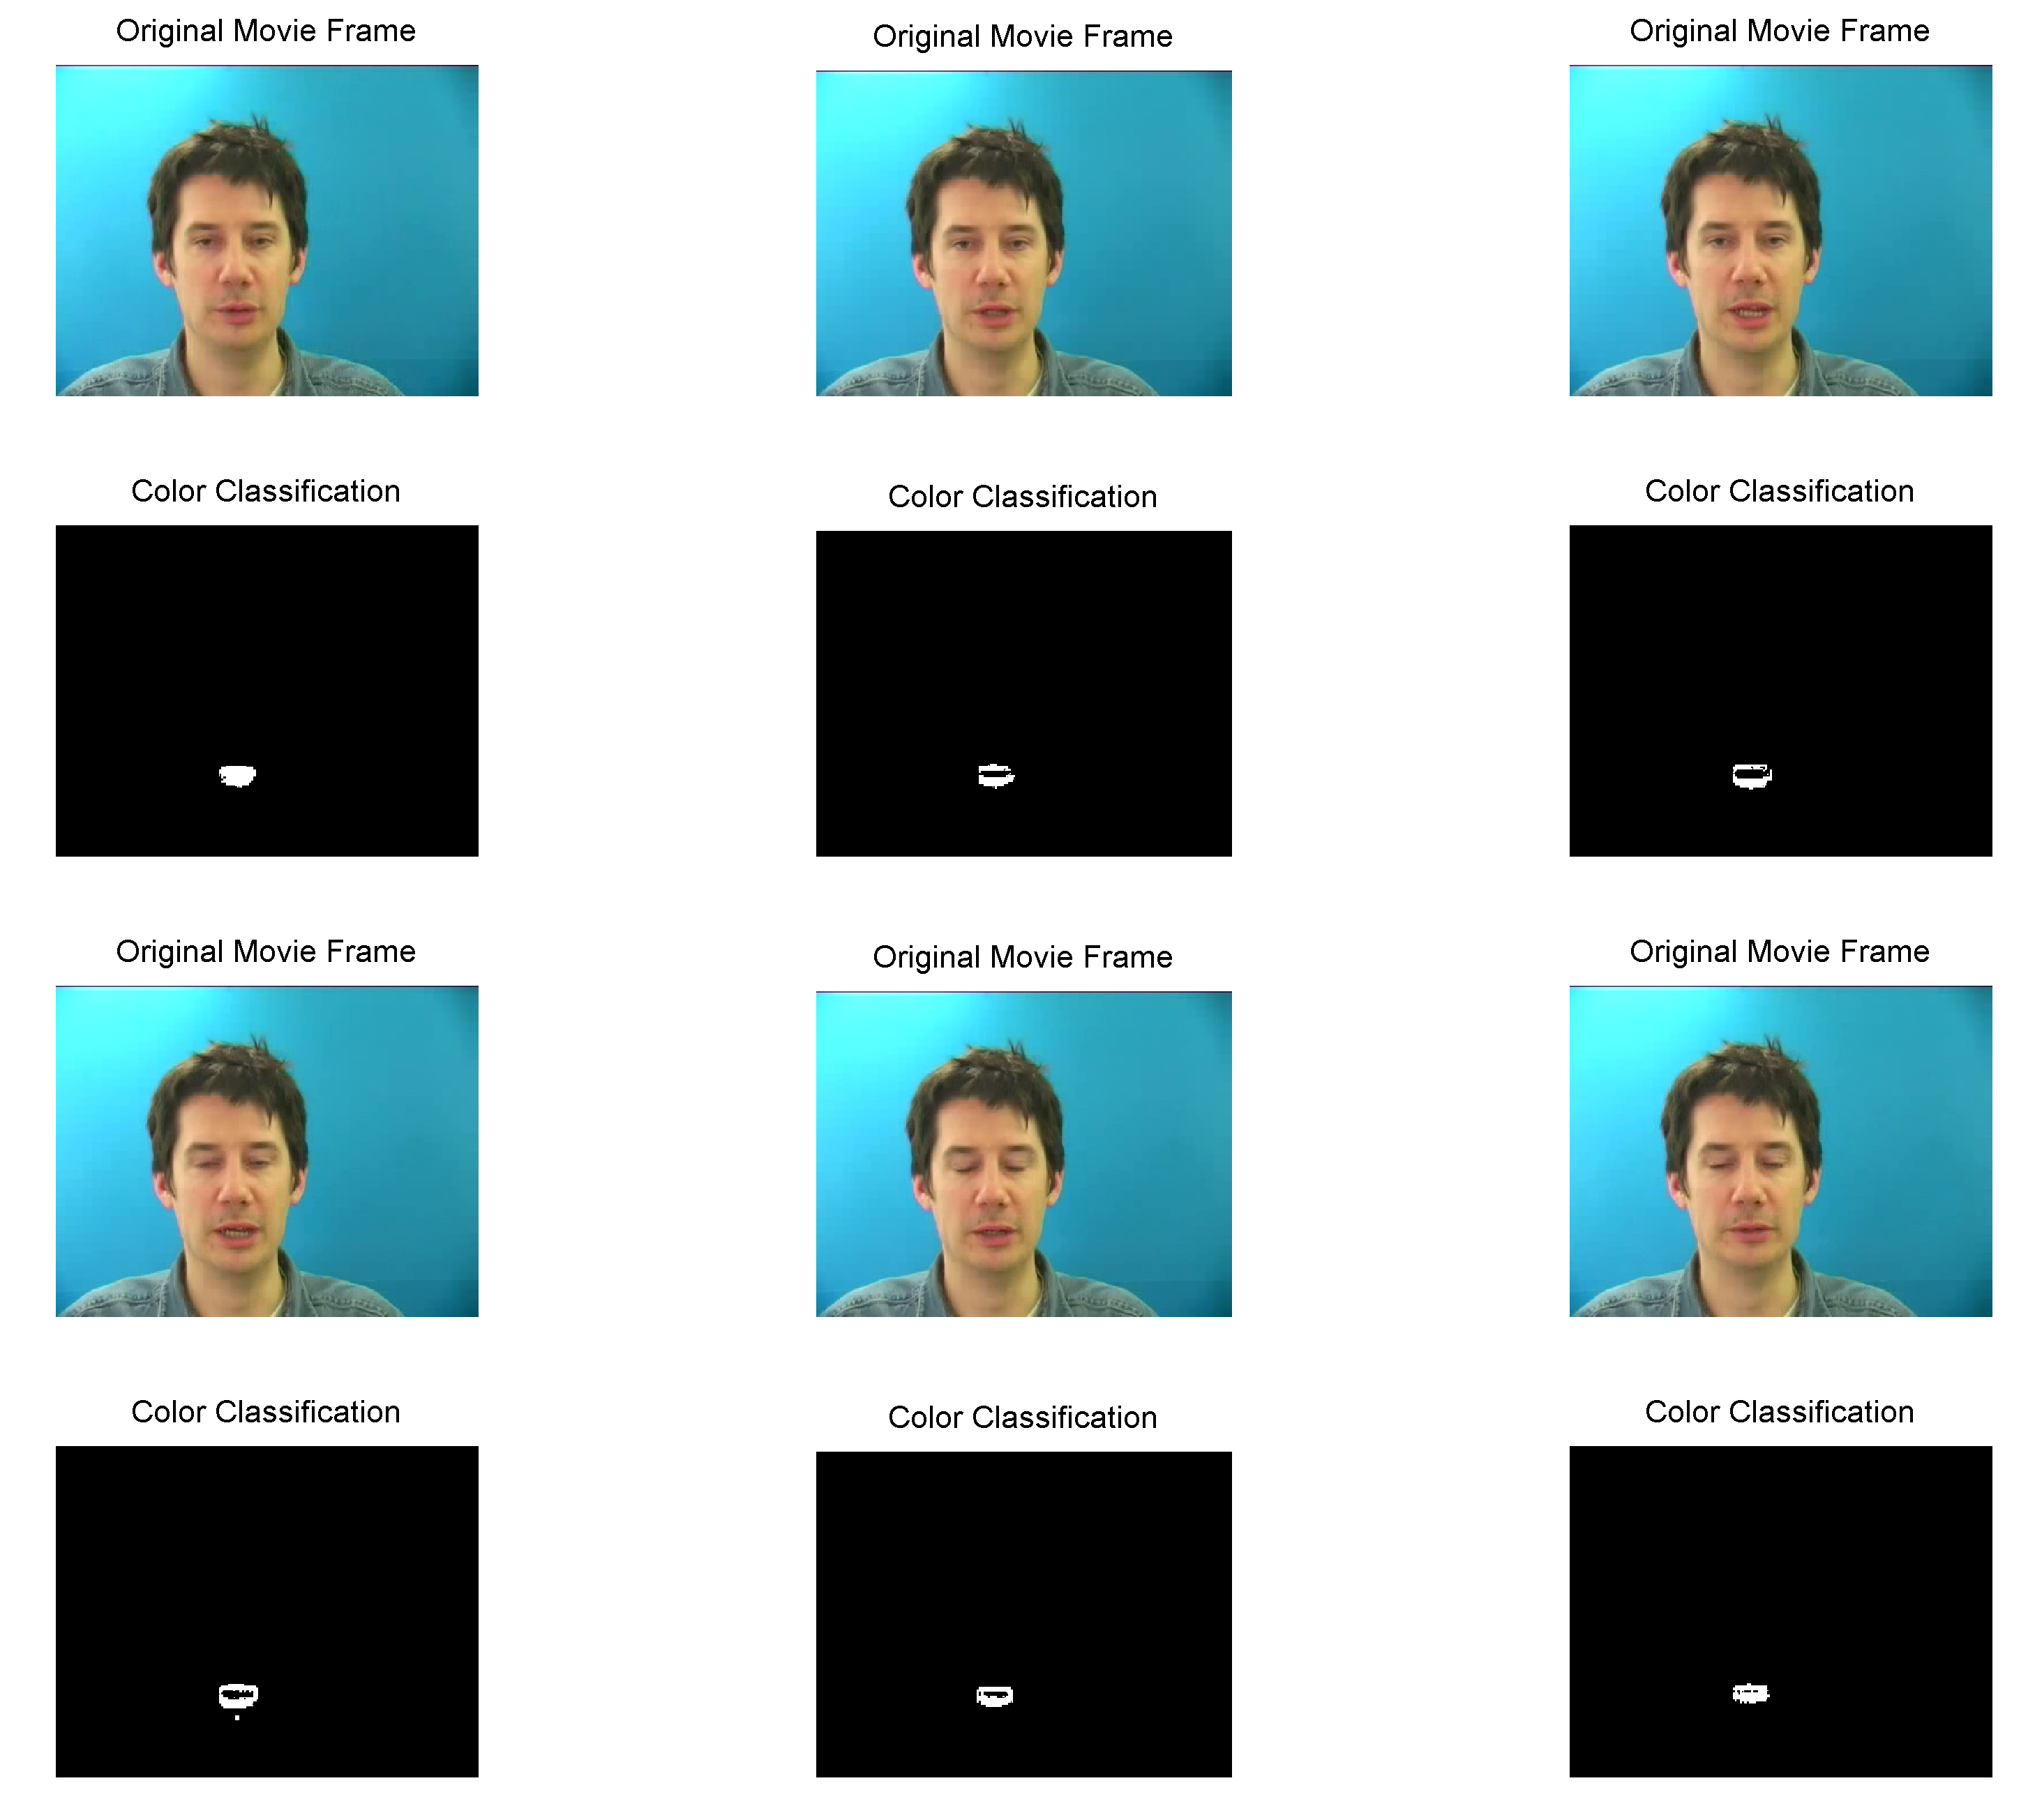
\includegraphics[width=1\textwidth]{color1.png}
	\caption{Color Classification for selected frames. Arguably the best overall method for capturing the movement of the lips.}
\end{figure}

\begin{figure}
	\centering
	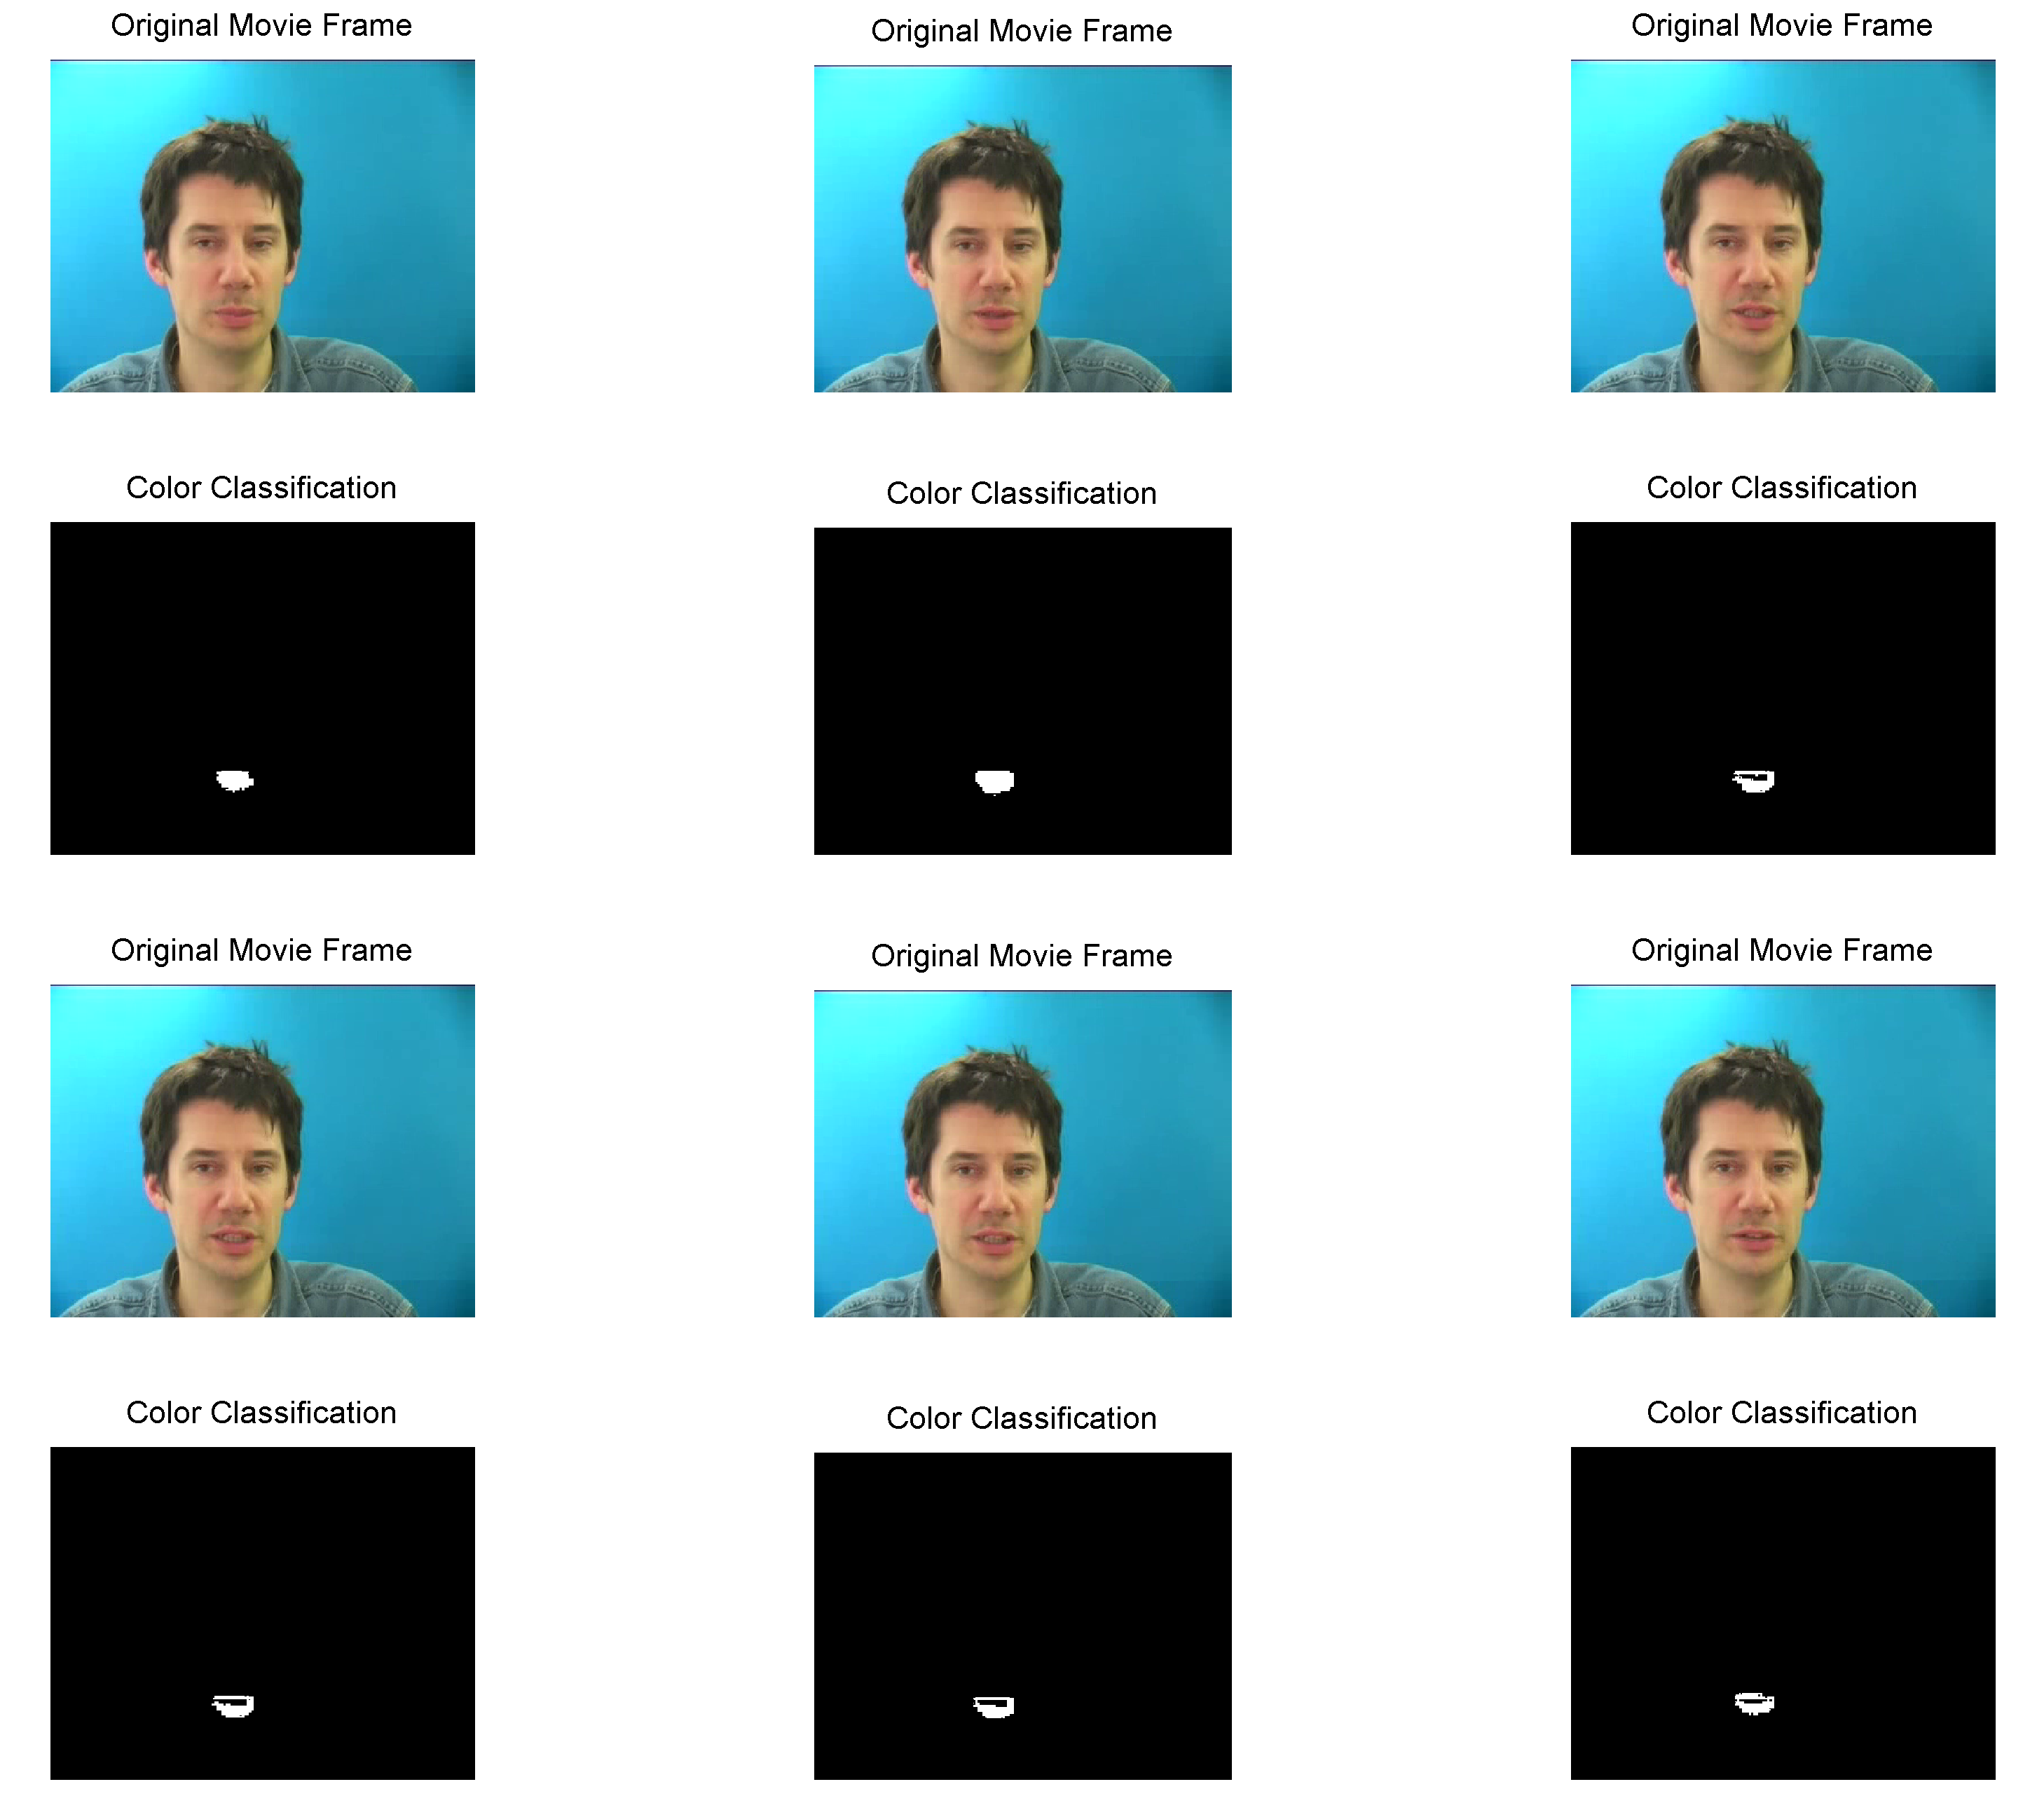
\includegraphics[width=0.5\textwidth]{color2.png}
	\caption{Color Classification for selected frames. Arguably the best overall method for capturing the movement of the lips.}
\end{figure}

\section*{Abstract}
The goal of this project is to develop a limited lip reading algorithm for a subset of the english language. We consider a scenario in which no audio information is available. We first develop a method for processing raw video and extracting the position of the lips in each frame. We then prepare the lip data for processing and classify the lips into visemes and phonemes. We then use Hidden Markov Models to predict the words the speaker is saying based on  the classification. We use the GRID audiovisual sentence corpus database for our study. 

\section{Introduction}
We consider 4 different algorithms for extracting the lip position. \begin{itemize}
  \item Active Contour Mask (Matlab built in)
\item Dynamic Mode Decomposition 
\item Edge Detection (Matlab built in)
\item Color Classification
\end{itemize}
We apply these techniques on a group of 1000 videos of a single speaker from the GRID audiovisual sentence corpus database. Each video is 3 second long and contains the speaker saying a number of nonsense phrases. The phrases spoken are chosen to convey a variety of sounds and therefore lip positions.



\section{Theoretical Development}
Lip reading is a complicated task and there are no "go-to" algorithms for detecting and tracking the position of an individual's lips. We can use Matlab's built in active contour and edge detection to hope to do background/foreground seperation on the video. We can also use DMD to do background/foreground seperation. The assumption is the speaker's face is stationary enough that it is possible to detect the lips as the foreground. In practice, this is not the case. We can also classify the pixel colors of the video frames and segment the lips based on the idea that the speaker's lip color is different from their skin color. For color classification, we can project the pixel color into the LAB color space to acheive better classification results. In either of these different strategies we also need to isolate the general mouth region of the speaker so that we will not also detect eyes, nose, etc. 

\section{Algorithm Development}

We can experiment with the different segmentation types for Matlab's active contour and edge detection. For active contour, Chan-Vese gives poor results with irregular edges. Edge method for active contour gives smoother regions but irregular shapes. Active contour takes many iterations to properly converge and gives poor results. Matlab's built in edge detection has many different methods as well. Sobel, Canny,


\end{document}

































